%%%%%%%%%%%%%%%%%%%%%%%%%%%%%%%%%%%%%%%%%%%%%%%%%%%%%%%%%%%%%%%%%%%%%%%%%%%
\documentclass[12pt]{article}
\usepackage{pdfpages}
\usepackage{graphicx}
\usepackage{epstopdf}
\usepackage{epsfig}
\usepackage{float}
\usepackage{graphicx}% Include figure files
%\usepackage{cite}
%\usepackage{rotating}% Include figure files
\usepackage{dcolumn}% Align table columns on decimal point
\usepackage{bm}% bold math
\usepackage{tabularx}
\usepackage{hyperref}
%\usepackage{mciteplus}
\usepackage[utf8]{inputenc}
\usepackage{amssymb}
\usepackage{subfigure}
\usepackage{amsmath}
\usepackage{multirow}
%\usepackage{multicol}
%\usepackage{booktabs}
\usepackage{xspace}
\usepackage{booktabs}
\usepackage{sidecap}   % sidecaptions
\usepackage{subfigure}
\usepackage{ulem} % strikeout
\usepackage{array}
\usepackage{xcolor}
\usepackage[titletoc]{appendix}
\usepackage{rotating}
\usepackage{lipsum}  
\usepackage{comment}
\usepackage{subfiles} %To work with multiple tex files in project
\usepackage{algorithm}
\usepackage{algpseudocodex}
%\usepackage[utf8]{inputenc}
%\usepackage[T1]{fontenc}
\usepackage [english]{babel}
\usepackage [autostyle, english = american]{csquotes}
\usepackage{bm}
\MakeOuterQuote{"}
%%%%%%%%%%%%%%%%%%%%%%%%%%%%%%%
\setlength{\textwidth}{18.0cm}
\setlength{\textheight}{23.0cm}
\setlength{\oddsidemargin}{0.0cm}
\setlength{\evensidemargin}{0.0cm}
\setlength{\headheight}{0cm}
\setlength{\headsep}{0cm}
\setlength{\topmargin}{0.0cm}
\setlength{\footskip}{1.5cm}
%%%%%%%%%%%%%%%%%%%%%%%%%%%%%
\renewcommand{\baselinestretch}{1.3}
%\usepackage[style=numeric-comp,sorting=none]{biblatex}%<- specify style
%\addbibresource{ref.bib}
\usepackage{listings}
\usepackage{xcolor}

\definecolor{codegreen}{rgb}{0,0.6,0}
\definecolor{codegray}{rgb}{0.5,0.5,0.5}
\definecolor{codepurple}{rgb}{0.58,0,0.82}
\definecolor{backcolour}{rgb}{0.95,0.95,0.92}

\lstdefinestyle{mystyle}{
    backgroundcolor=\color{backcolour},   
    commentstyle=\color{codegreen},
    keywordstyle=\color{magenta},
    numberstyle=\tiny\color{codegray},
    stringstyle=\color{codepurple},
    basicstyle=\ttfamily\footnotesize,
    breakatwhitespace=false,         
    breaklines=true,                 
    captionpos=b,                    
    keepspaces=true,                 
    numbers=left,                    
    numbersep=5pt,                  
    showspaces=false,                
    showstringspaces=false,
    showtabs=false,                  
    tabsize=2
}

\lstset{style=mystyle}

%%%%%%%%%%%%%%%%%%%%%%%%%%%
\begin{document}
\baselineskip 0.7cm
\title{\bf \color{blue}Lotka Volterra Predator Prey Model }
\vskip 3cm
\author{Pawanpreet Kaur \\ (2020PHY1092) \and 
Preetpal Singh \\ (2020PHY1140) \and 
Anjali \\ (2020PHY1164) \\
{\color{blue}S.G.T.B. Khalsa College, University of
Delhi, Delhi-110007, India.} }

\maketitle
\vskip 4cm
\begin{center}
{\it {\color{blue}Project Report Submitted to}}\\
Dr. Mamta and Dr. H. C. Ramo \\
\textit{\color{blue}as part of internal assessment for the course}\\
 "32223902 - Computational Physics Skills"
\end{center}

\pagenumbering{gobble}

\newpage
%\vskip 1cm

\pagenumbering{roman}
\abstract{Predator-prey models are arguably the building blocks of the bio- and ecosystems as biomasses are grown out of their resource masses. Species compete, evolve and disperse simply for the purpose of seeking resources to sustain their struggle for their very existence.\newline One of the most ecological applications of differential equations systems is
predator-prey problem. In fact, differential equations are very useful in many
areas of applied sciences. However, most of the nature problems involve with
some unknown function. In this paper, an environmental case containing two
related populations of prey species and predator species is studied. It is expected
that two population make influence on the size of each other. Since it involves some assumptions, so this model is quite unrealistic.\newline}
%\abstract{\lipsum[1-1]}
\newpage
\tableofcontents
\newpage

\pagenumbering{arabic}
\section{Introduction}
\label{sec:intro}
\section*{Motivation}
As differential equations are one of the most important concepts related to analyse real life phenomenas. We are doing Lotka Volterra Model because it gives us glimpse predator and pre their interaction works and interestingly gives us mathematical formulation through which we can make predictions to take legitimite actions to make this wildlife balance. \\

\subsection*{History\cite{noauthor_lotkavolterra_nodate}}
In the 1920s, the Italian mathematician Vito Volterra proposed a differential equations model to describe the population dynamics of two interacting
species of a predator and its prey. He hoped to explain the increasing in predator fish (and so,decreasing in prey fish) in the Adriatic Sea during World War
I. Independently, these equations studied by Volterra were derived by Alfred Lotka to describe a hypothetical chemical reaction in which the chemical
concentrations oscillate , in the United States. There are many species of
animals in nature where one species feeds on another species. The first species
and the second one are called predator and prey respectively.\\

\subsection*{Lotka Volterra Model}
The Lotka-Volterra equations, also known as predator-prey equations, were developed to describe the dynamics of biological systems. This system of non-linear differential equations can be described as a more general version of a Kolmogorov model\cite{noauthor_kolmogorov_nodate} because it focuses only on the predator-prey interactions and ignores competition, disease, and mutualism which the Kolmogorov model includes. \par The Lotka-Volterra equations can be written simply as a system of first-order non-linear ordinary differential equations (ODEs). Since the equations are differential in nature, the solutions are deterministic (no randomness is involved, and the same initial conditions will produce the same outcome), and the time is continuous (the generations of predators and prey are continually overlapping). 
\newpage

\subsection*{Predator Prey Equations\cite{noauthor_lotkavolterra_nodate}}
The model satisfies the
system of ODEs: \\
\begin{equation*}
\frac { d x } { d t } = x ( \alpha - \beta y )
\end{equation*}
\begin{equation*}
\frac { d y } { d t } = - y ( \gamma - \delta x )
\end{equation*}

where,
\begin{itemize}
    \item x is the number of prey.
    \item y is the number of some predator.
    \item $ \frac { d y } { d t } $ and $ \frac { d x } { d t } $ represent the growth rates of the two populations over time
    \item t represents time.
    \item $ \alpha , \beta , \gamma $ and $ \delta $ are parameters describing the interaction of the two species.
\end{itemize}
\
\newline Last paragraph should contain plan of the report - one sentence about each of the following sections.
\newpage

%%%%%%%%%%%%%%%%%%%%%%%%%%%%%%%%%%%%%%%%%%%%%%%%
\section{Theory}
\label{sec:theory}
\subsection*{Problem}
In this project, we analyse Lotka-Volterra Predator-Prey Model that describe the interaction between predator and prey in given environment with some assumptions. With the help of this model we predict the number of predator and preys at particular time in future from the point where we consider our data. So, we analyse our results with different numerical methods and plotting techniques.
\subsection*{Assumptions made for the Model}
To keep the model simple,  some assumptions are made that would be unrealistic in most of the predator-prey situations in real world. Specifically, it is assumed that
\begin{enumerate}
    \item Only two species exist : Predator and Prey.
    \item The prey population finds ample food at all times and are born and then die through predation or inherent death.
    \item Predators have limitless appetite and they are born and their birth rate is positively affected by the rate of predation, and they die naturally.
    \item The food supply of the predator population depends entirely on the size of the prey population.
    \item The rate of change of population is proportional to its size.
    \item During the process, the environment does not change in favour of one species and the genetic adaptation is sufficiently slow.
\end{enumerate}
\subsection*{Description of Parameters}
\begin{itemize}
    \item $\alpha$ is the growth rate of species x (the prey) in the absence of interaction with species y (the predators)
    \item $\beta$ measures the impact of predation on $ \dot{x}/x $ (the rate at which predators destroy prey)
    \item $\delta$ denotes the net rate of growth (or immigration) of the predator population in response to the size of the prey population
    \item  $\gamma$ is the death (or emigration) rate of species y in the absence of interaction with species x
\end{itemize} 

\subsection*{Realistic Model}
Very few such “pure” predator-prey interactions have been observed in nature. A simplified interaction is seen in Canadian northern forests where populations of the lynx and the snowshoe hare are intertwined in a life and death struggle. There are good records of pelts of these species trappers brought to the Hudson Bay Company.

\begin{figure}[h] 
    \centering
    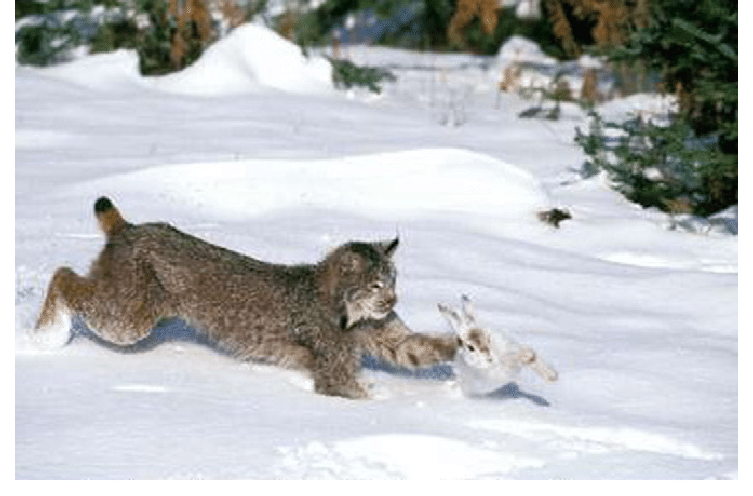
\includegraphics[width=15cm,height=12cm]{Photograph-of-Canadian-Lynx-and-Snowshoe-Hare-Balance-Problem-Used-in-Consolidity-Theory.png}
\caption{\bf{Lynx and Hare: Specialized tightly linked predator and prey relationship.\cite{noauthor_photograph_nodate}}}
\end{figure}
\newpage
\subsubsection*{Hudson Bay Company}
Detailed records on pelts were collected over almost 100 years. Below is data from 1900-1920.\cite{noauthor_untitled_nodate} \cite{noauthor_mathematical_nodate}
\begin{figure}[h] 
    \centering
    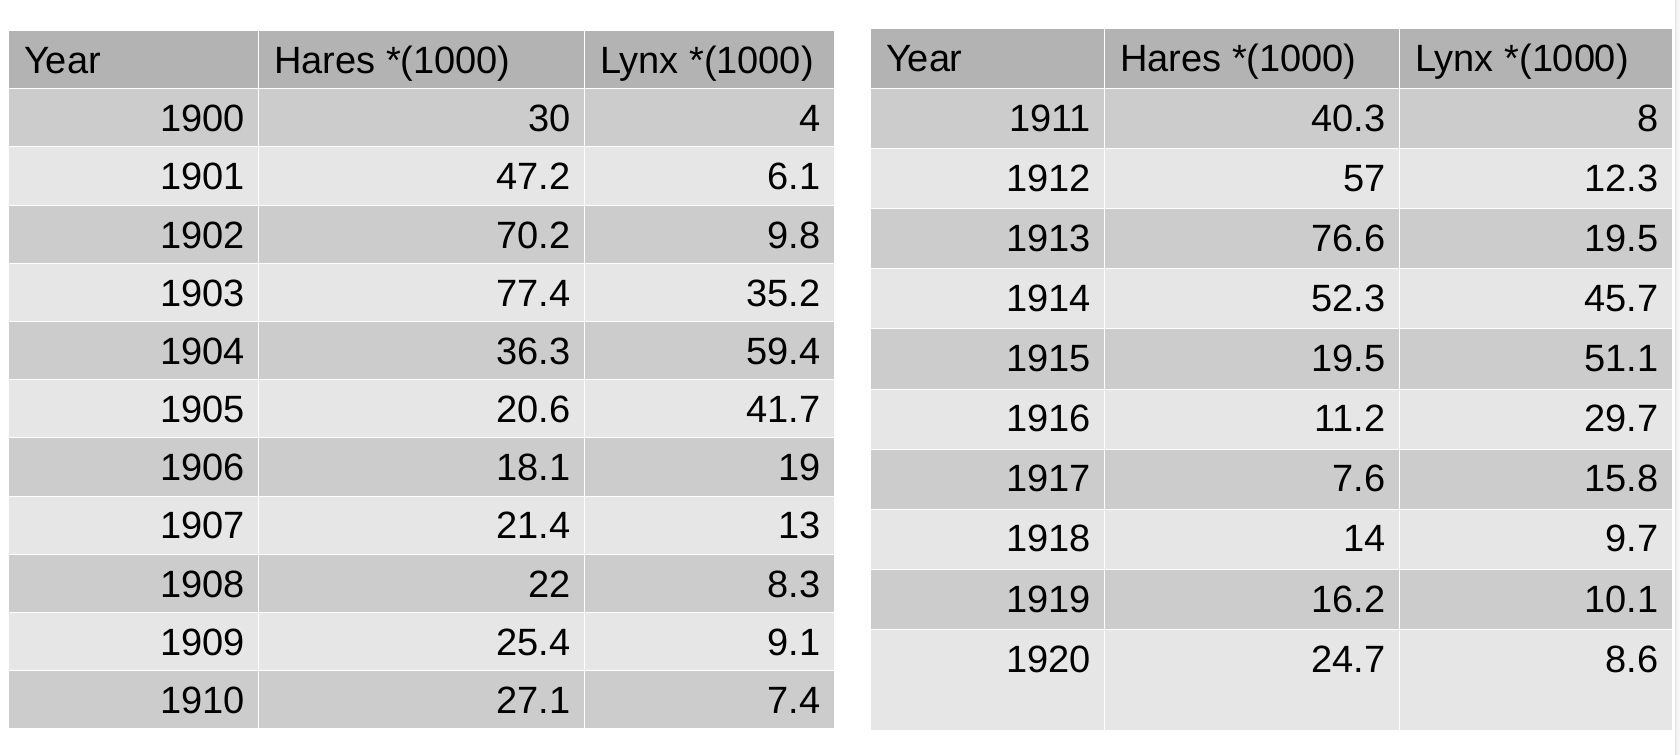
\includegraphics[width=15cm,height=12cm]{ss_tab.jpg}
\caption{Data from 1900-1920}
\end{figure}
\begin{itemize}
    \item Data from 1900-1920 show distinct rise of hares followed by a rise in lynx.
    \item Theory has predicted that following a rise of prey, then populations of predator increase.
    \item Develop Lotka-Volterra model exhibiting this behavior
    \item  This simplified system creates a good opportunity to create a mathematical model.
\end{itemize}
\section*{Mathematical Modelling}
\subsection*{Prey Equation}
\begin{equation*}
     \frac { d x } { d t } = \alpha x - \beta x y = f(x,y)
\end{equation*}

The prey are assumed to have an unlimited food supply, and to reproduce exponentially unless subject to predation;
this exponential growth is represented in the equation above by the term $ \alpha x . $ The rate of predation upon the prey is
assumed to be proportional to the rate at which the predators and the prey meet; this is represented above by $ \beta x y $. If
either $ x $ or $ y $ is zero then there can be no predation.

\subsection*{Predator Equation}
\begin{equation*}
    \frac { d y } { d t } = \delta x y - \gamma y = g(x,y)
\end{equation*}

In this equation, $ \delta x y $ represents the growth of the predator population. (Note the similarity to the predation rate;
however, a different constant is used as the rate at which the predator population grows is not necessarily equal to the
rate at which it consumes the prey). $ \gamma y $ represents the loss rate of the predators due to either natural death or
emigration; it leads to an exponential decay in the absence of prey.

\subsection*{Population Equilibrium($x_{eq},y_{eq})$}
Population equilibrium occurs in the model when neither of the population levels is changing, i.e. when both of the
derivatives are equal to $ 0 . $ These points are called critical points.
\begin{equation*}
    \frac { d y } { d t } = \delta x y - \gamma y = 0
\end{equation*}
\begin{equation*}
     \frac { d x } { d t } = \alpha x - \beta x y = 0
\end{equation*}

The possibilities are, 
\begin{itemize}
    \item $ y = 0 $ , $ x = 0 $ so $ y_{eq} = 0 $ , $ x_{eq} = 0 $
    \item \alpha - \beta y = 0 \Longrightarrow $y_{eq} = \frac{\alpha}{\beta}$ similarily $x_{eq} = \frac{\gamma}{\delta}$
\end{itemize}

\section*{Implementation of Linearisation for Predator-Prey \\ Problem \cite{noauthor_differential_nodate}} 

\begin{equation*}
    f ( x , y ) \approx f ( x_{eq} , y_{eq} ) + \left( \frac { \partial f } { \partial x } \right) ( x - x_{eq} ) + \left( \frac { \partial f } { \partial y } \right) ( y - y_{eq} )
\end{equation*}
\begin{equation*}
     g ( x , y ) \approx g ( x_{eq} , y_{eq} ) + \left( \frac { \partial g } { \partial x } \right) ( x - x_{eq} ) + \left( \frac { \partial g } { \partial y } \right) ( y - y_{eq} )
\end{equation*}

A critical point has $ f ( x_{eq} , y_{eq} ) = g ( x_{eq} , y_{eq} ) = 0 $. So, the equation becomes linear combination of x and y. So, the general equation becomes,

\begin{equation*}
    \left[ \begin{array} { c } ( x - x_{eq} ) ^ { \prime } \\ ( y - y_{eq} ) ^ { \prime } \end{array} \right] \approx \left[ \begin{array} { l l } \partial f / \partial x & \partial f / \partial y \\ \partial g / \partial x & \partial g / \partial y \end{array} \right] \left[ \begin{array} { c } x - x_{eq} \\ y - y_{eq} \end{array} \right] = J \left[ \begin{array} { c } x - x_{eq} \\ y - y_{eq} \end{array} \right] 
\end{equation*}

\subsection*{Implementation of Linearisation for Predator-Prey Problem}

The critical points are (0,0) and ($\frac{\gamma}{\delta}$,$\frac{\alpha}{\beta}$) \\
\subsubsection*{First critical point}
At $x_{eq}, y_{eq} = (0,0)$ \\

\begin{equation*}
J = \left[ \begin{array} { l l } \partial f / \partial x & \partial f / \partial y \\ \partial g / \partial x & \partial g / \partial y \end{array} \right] = \left[ \begin{array} { c c } \alpha - \beta y_{eq} & - \beta x_{eq} \\ \delta y_{eq} & \delta x_{eq} - \gamma \end{array} \right] = \left[ \begin{array} { c c } \alpha & 0 \\ 0 & - \gamma \end{array} \right]
    
\end{equation*}
The eigenvalues of this matrix are $ \lambda _ { 1 } = \alpha , \quad \lambda _ { 2 } = - \gamma $. As the eigen values are oppsoite in sign and always greater than zero, so the fixed point near origin will be saddle point. Near critical point (0,0) the baboon's population $ x ( t ) $ will grow but the population of cheetahs $y(t)$ will decay. It can only happen when there is very less interaction between predator and prey. So, extinction can only happen when prey are artifically eradicated due to which cheetahs will die due to natural reasons(starvation etc).

\begin{equation*}
    \left[\begin{array} { c } \frac { d x ( t ) } { d t } \\ \frac { d y ( t ) } { d t } \end{array} \right] = c _ { 1 } \left[ \begin{array} { l } 1 \\ 0 \end{array} \right] e ^ { \alpha t } + c _ { 2 } \left[ \begin{array} { l } 0 \\ 1 \end{array} \right] e ^ { - \gamma t } 
\end{equation*}



\subsubsection*{Second Critical Point}
At (x_{eq}, y_{eq})=($\frac{\gamma}{\delta}$,$\frac{\alpha}{\beta}$) \\

\begin{equation*}
    J \left( \frac { \gamma } { \delta } , \frac { \alpha } { \beta } \right) = \left[ \begin{array} { l l } \partial f / \partial x & \partial f / \partial y \\ \partial g / \partial x & \partial g / \partial y \end{array} \right] = \left[ \begin{array} { c c } \alpha - \beta y_{eq} & - \beta x_{eq} \\ \delta y_{eq} & \delta x_{eq} - \gamma \end{array} \right] = \left[ \begin{array} { c c } 0 & - \frac { \beta \gamma } { \delta } \\ \frac { \alpha \delta } { \beta } & 0 \end{array} \right]
\end{equation*}


The eigenvalues of this matrix are
$ \lambda _ { 1 } = i \sqrt { \alpha \gamma } = +i \omega , \quad \lambda _ { 2 } = - i \sqrt { \alpha \gamma } = - i \omega. $
Because the real part is zero, so the stability is neutral and critical points are center. The solution will form closed trajectories surrounding the critical point(1,1). Consequently, the levels of
the predator and prey populations cycle, and oscillate around this fixed point.

Extra baboons $ \rightarrow $ Cheetahs increase $ \rightarrow $ Baboons decrease $ \rightarrow $ Cheetahs decrease $ \rightarrow $ Extra Baboons

\begin{equation*}
     \left[\begin{array} { c } \frac { d x ( t ) } { d t } \\ \frac { d y ( t ) } { d t } \end{array} \right] = c _ { 1 } \left[\begin{array} { c } \cos ( \omega t ) \\ A \sin ( \omega t ) \end{array} \right] + c _ { 2 } \left[ \begin{array} { c } \sin ( \omega t ) \\ - A \cos ( \omega t ) \end{array} \right]
\end{equation*}
where,
\begin{equation*}
    A = \frac { \delta } { \beta } \sqrt { \frac { \alpha } { \gamma } }
\end{equation*}
To check whether the solution forms a perfect circle we will solve for $ \frac { d x} { d y } $ with separation of variables.

\begin{equation*}
    \frac { d x } { d y } = \frac { d x / d t } { d y / d t } = \frac { f } { g } = \frac  { x(\alpha  - \beta  y)} { y(\delta x  - \gamma )}
\end{equation*}
gives,
\begin{equation*}
    \frac { \delta x - \gamma}{x}  d x = \frac  {\alpha - \beta y }{ y } d y
\end{equation*}
\begin{equation*}
     \frac  {\alpha - \beta y }{ y } d y - \frac { \delta x - \gamma}{x}  d x = 0
\end{equation*}
Integrating on both sides with respect to y and x gives
\begin{equation*}
      Q(x,y) = \alpha \ln ( y ) - \beta y + \gamma \ln ( x ) - \delta x   = C
\end{equation*}


%%%%%%%%%%%%%%%%%%%%%%%%%%%%%%%%%
\newpage
\section{Methodology}
\label{sec:method}
Numerical Methods: Euler, Rk2, Rk4\\
\textbf{Inbuilt Numerical Method}: scipy.integrate.odeint \cite{noauthor_scipyintegrateodeint_nodate}

\subsection{Algorihtms}
\subfile{algorithm.tex}

%%%%%%%%%%%%%%%%%%%%%%%%%%%%%%%%%%%%%%
\newpage
\section{Analysis of Numerical Results}
Include all graphs, tables and analysis of the results. This should be a detailed section. 

\begin{figure}[h] %Euler for diff h
    \centering
    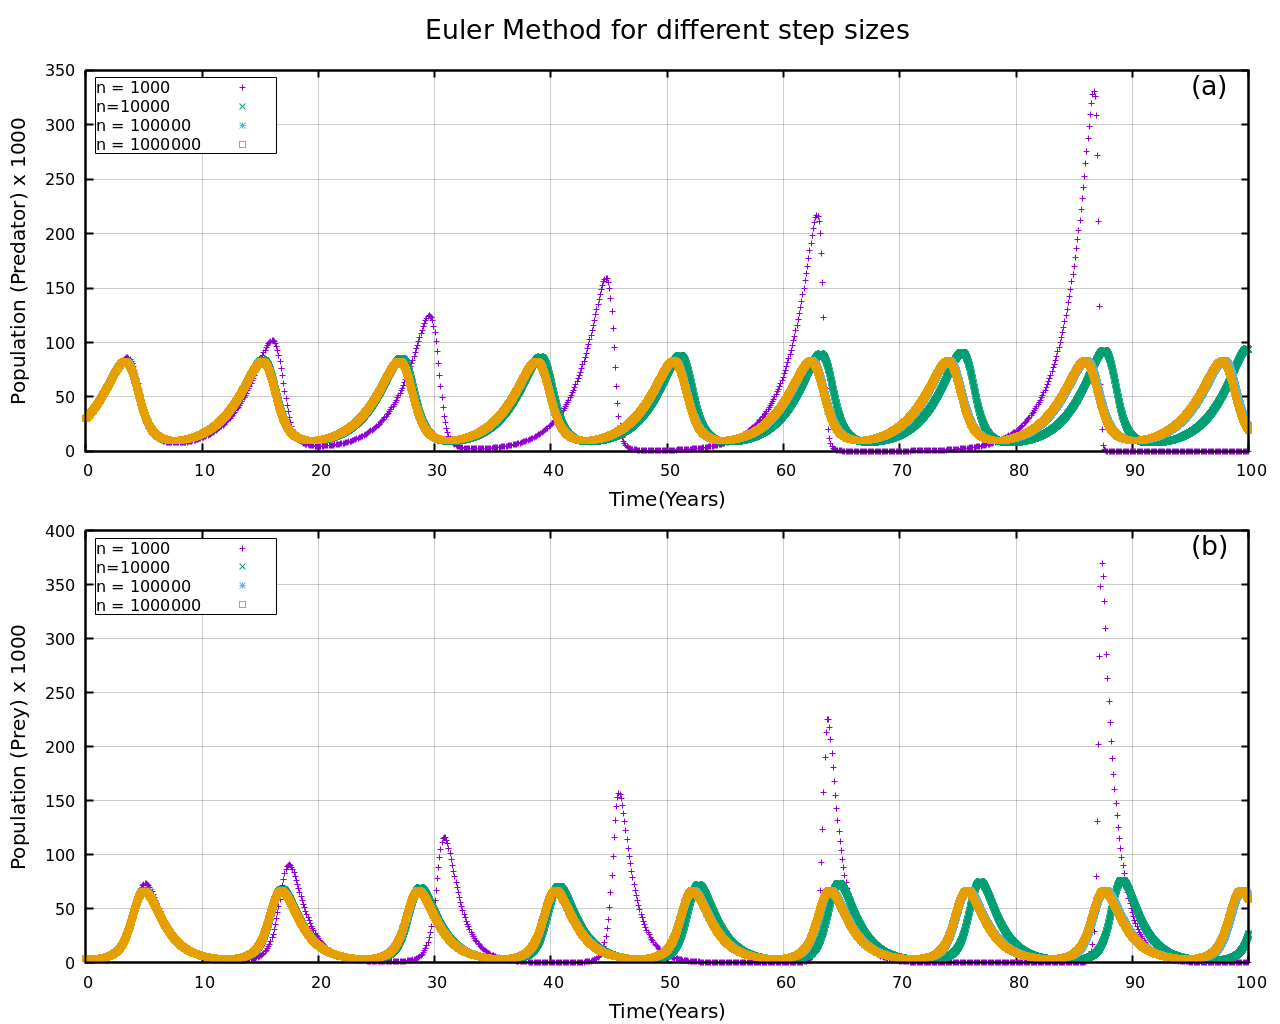
\includegraphics[width=15cm,height=12cm]{euler_diff_h.png}
\caption{\textbf{Euler Method For different step sizes:} $+$ symbol in purple color for 1000 data points, $\times$ symbol in green 10000, * symbol in sky blue 100000 and $\square$ symbol in mustard for 1000000 data points respectively.The results for Euler's Method converge for N=100000.\newline \textbf{SubFig(a):} Population of Predator v/s time(years), \textbf{SubFig(b):} Population of Prey v/s time(years)  }
\end{figure}

\newpage
\begin{figure}[h] %rk2 for diff h
    \centering
    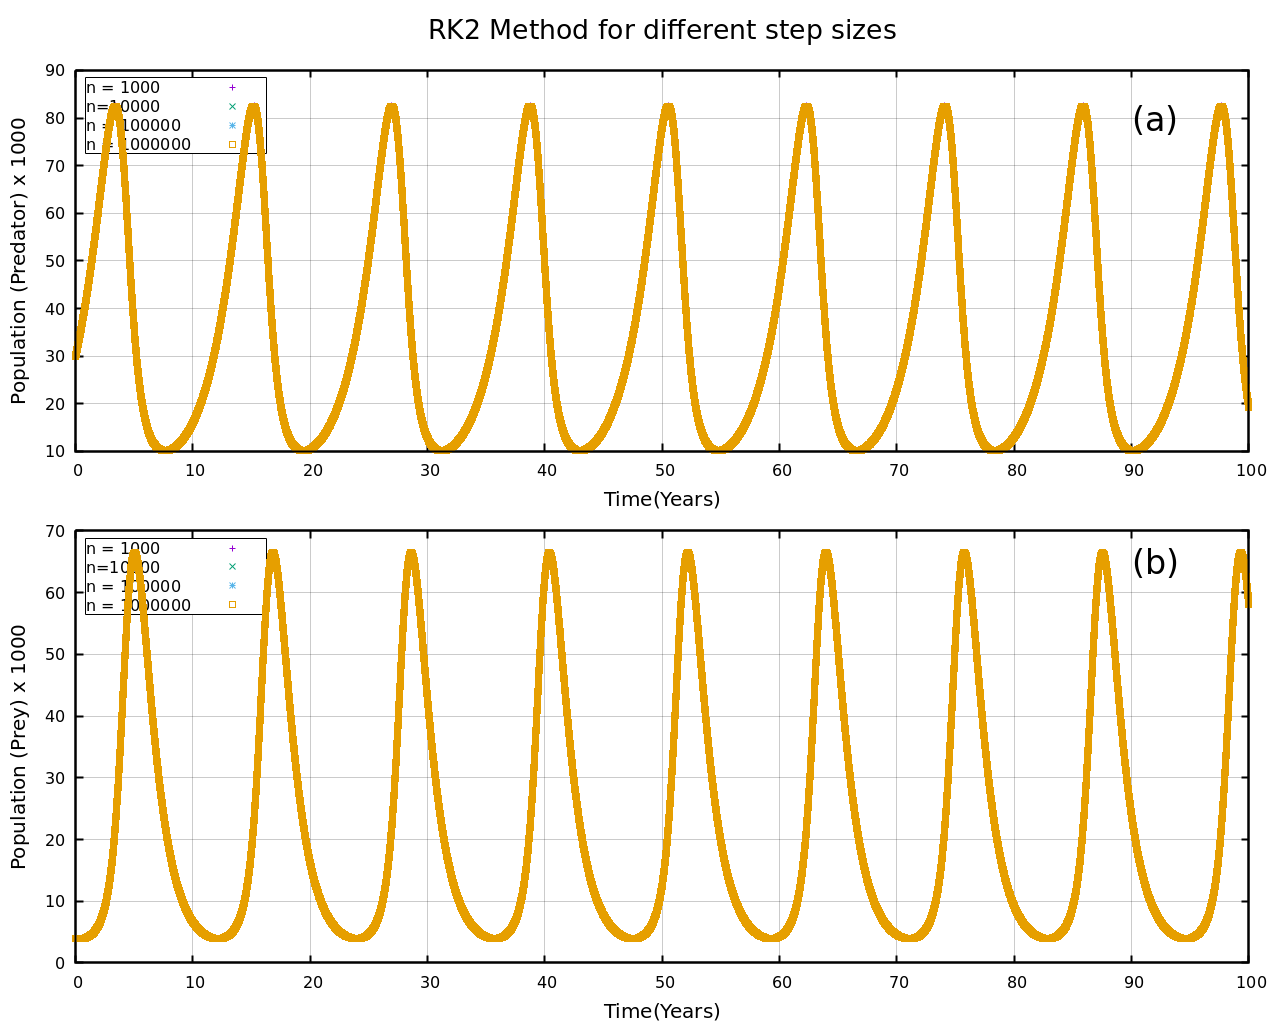
\includegraphics[width=15cm,height=12cm]{rk2_diff_h.png}
\caption{\textbf{RK2 Method For different step sizes:} $+$ symbol in purple color for 1000 data points, $\times$ symbol in green 10000, * symbol in sky blue 100000 and $\square$ symbol in mustard for 1000000 data points respectively.The results for RK2 Method converge for N=1000.\newline \textbf{SubFig(a):} Population of Predator v/s time(years), \textbf{SubFig(b):} Population of Prey v/s time(years)  }
\end{figure}

\newpage
\begin{figure}[h] %RK4 for diff h
    \centering
    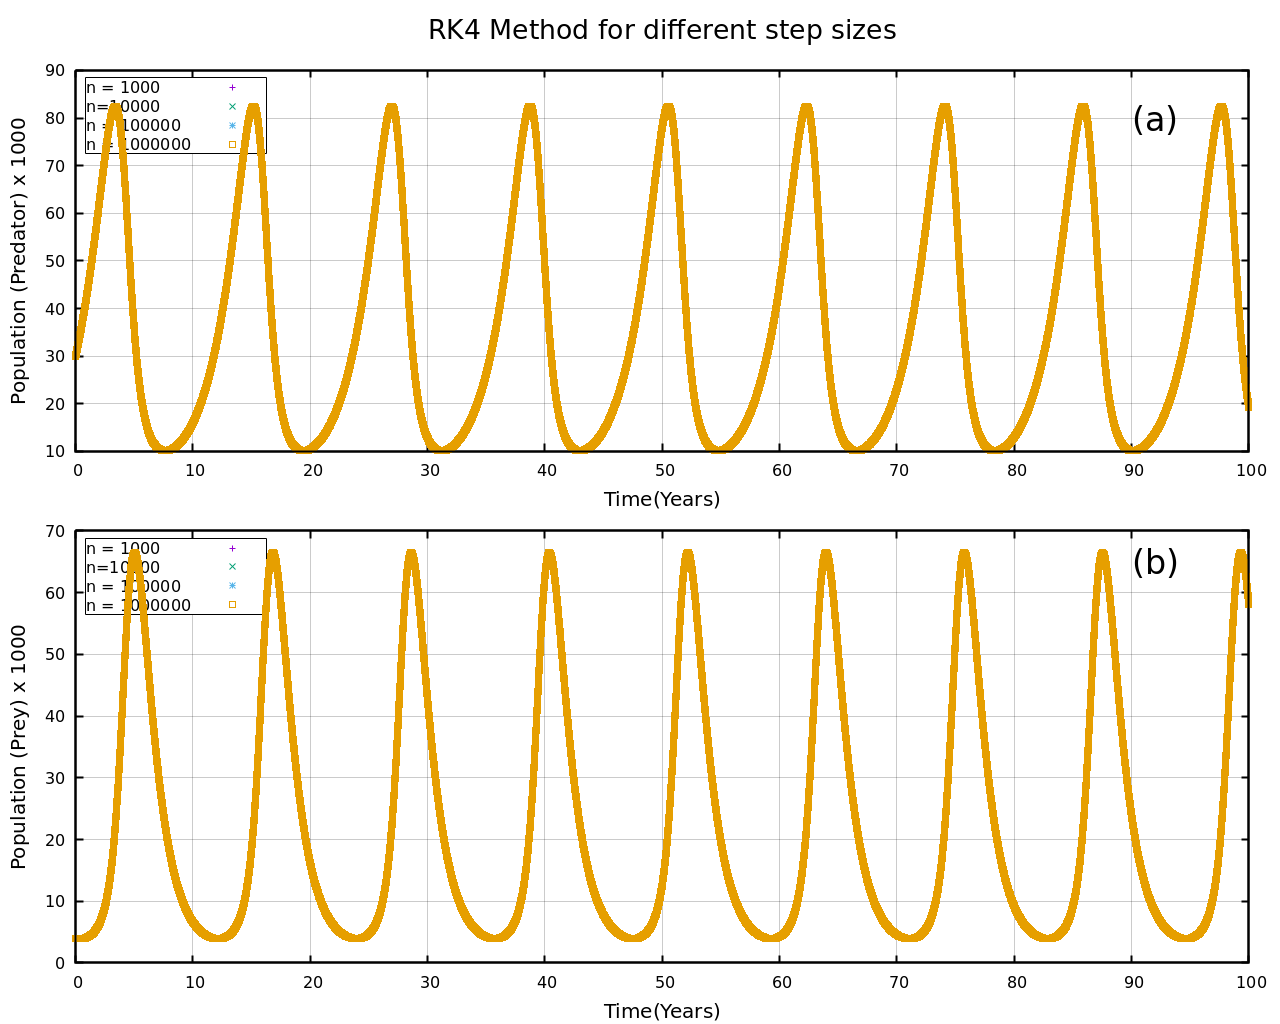
\includegraphics[width=15cm,height=12cm]{rk4_diff_h.png}
\caption{\textbf{RK4 Method For different step sizes:} $+$ symbol in purple color for 1000 data points, $\times$ symbol in green 10000, * symbol in sky blue 100000 and $\square$ symbol in mustard for 1000000 data points respectively. The results for RK4 Method converge for N=1000.\newline \textbf{SubFig(a):} Population of Predator v/s time(years), \textbf{SubFig(b):} Population of Prey v/s time(years)  }
\end{figure}
\newpage
\begin{figure}[h]
    \centering
    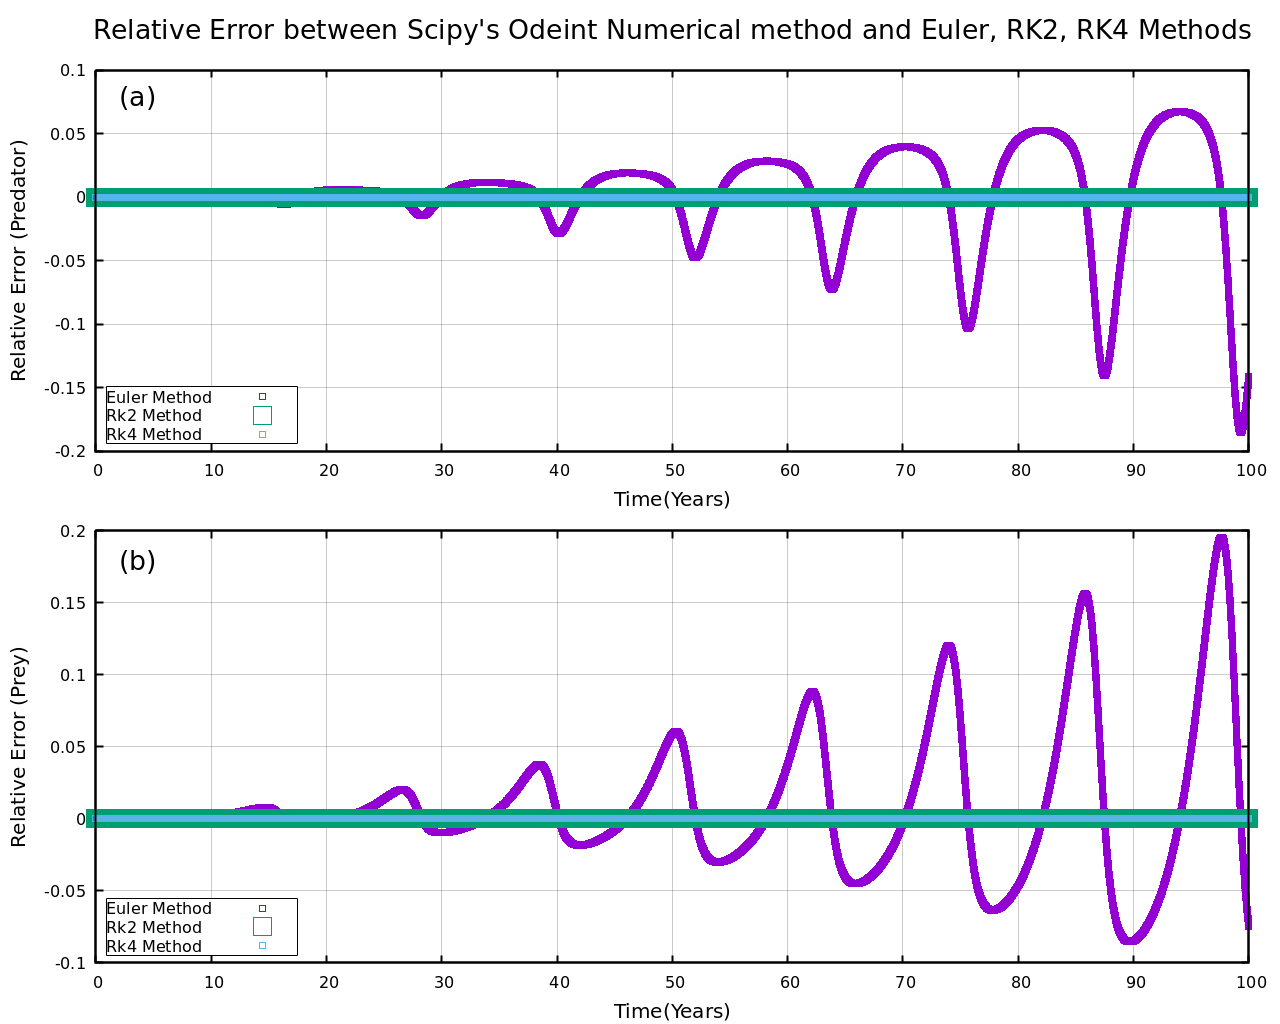
\includegraphics[width=15cm,height=12cm]{error_plot.png}
\caption{\textbf{Euler Method:} 100000 data points; \textbf{RK2 Method:} 10000 data points and \textbf{RK4 Method:} 1000 data points. The results of Euler's Method  won't converge with odeint(inbuilt) method because of the limitations of Euler's Method and function's oscillatory behaviour but it converges for RK2 and RK4 Method}
\end{figure}

\newpage
\begin{figure}[h] 
    \centering
    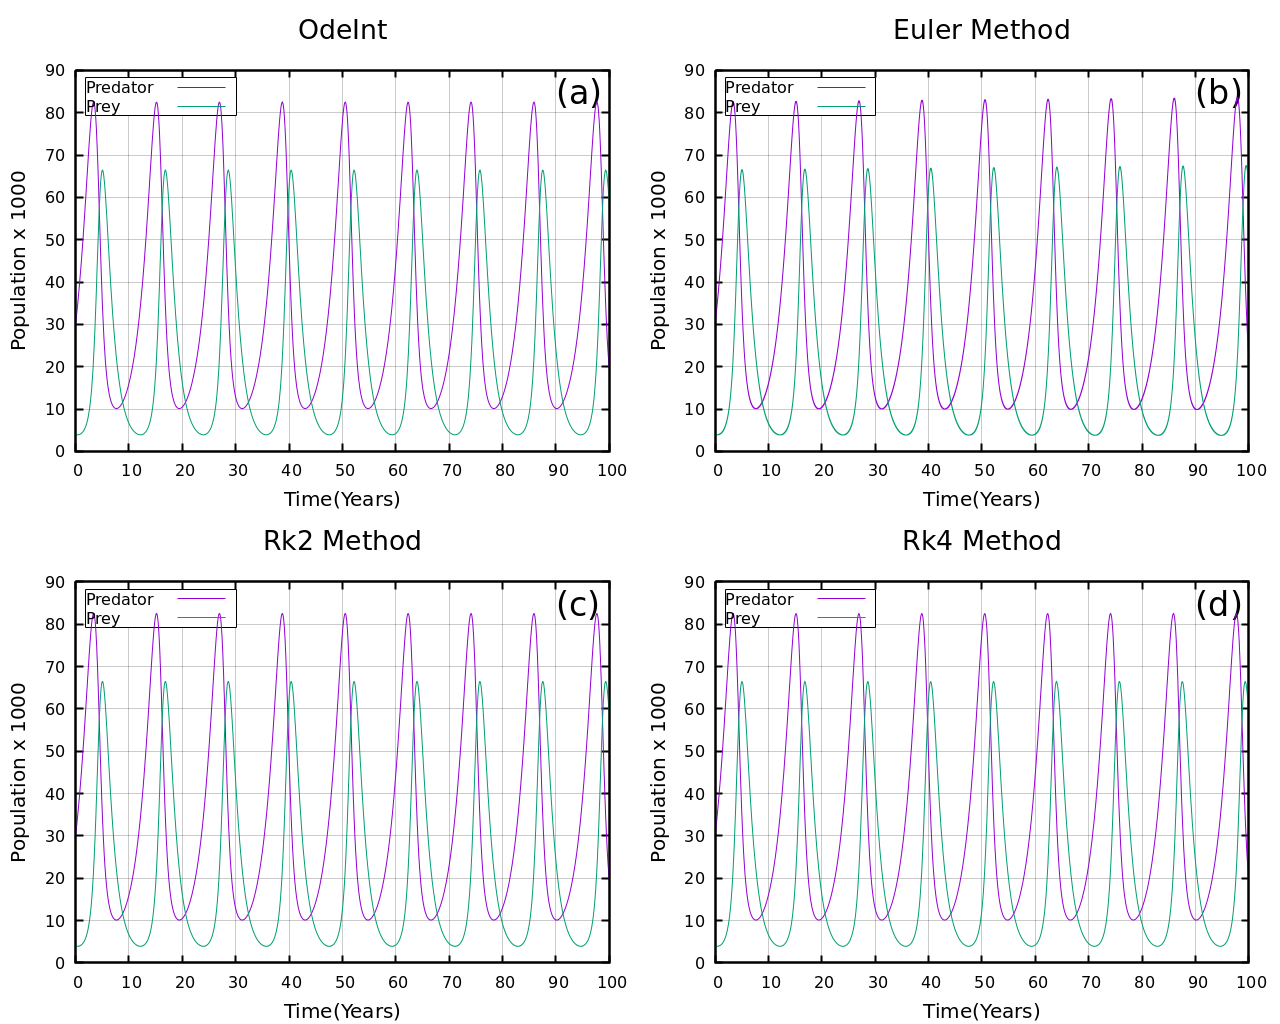
\includegraphics[width=18cm,height=15cm]{time_vs_population.png} 
\caption{Time v/s Population \textbf{Euler Method:} 100000 data points; \textbf{RK2 Method:} 10000 data points and \textbf{RK4 Method:} 1000 data points }
\end{figure}
Looking at the results of the simulation we can see that as the population of the prey 
begins the rise, the number of predators also begins to rise till the point at which predators kill 
off the prey faster than they can reproduce. Then the numbers begin to fall for the prey which 
thus causes a lack of food for the predators which numbers also begin to decline. The solution to 
this simulation is periodic meaning that the cycle will continue ad infinitum with the rise and fall 
of both populations. This looks very similar to the solution of simple harmonic motion, such as 
an un-damped spring-mass system except for the addition of a secondary plot.


\newpage
\begin{figure}[h] %Euler for diff h
    \centering
    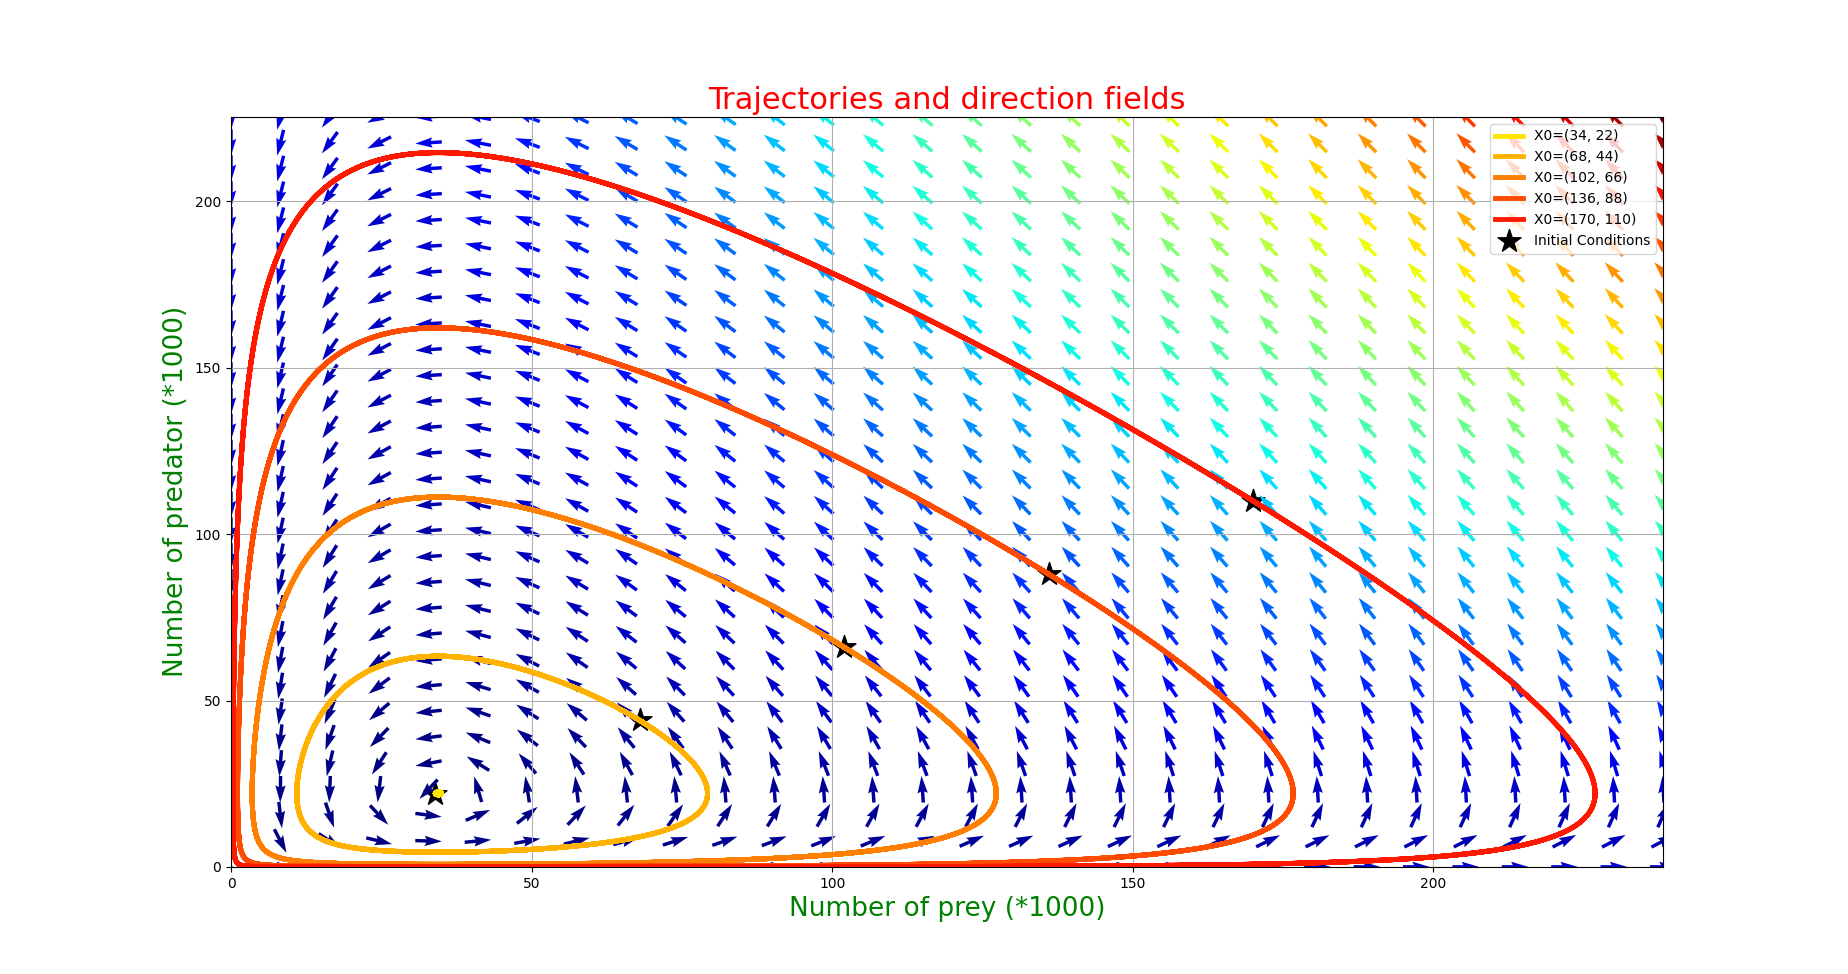
\includegraphics[width=18cm,height=13cm]{Trajcec_DirFields.png}
\caption{\textbf{Trajectories and Direction fields:} Phase-space plot for the predator prey problem for various initial conditions of the prey and predator population. The contours describe solutions of the system determined by their initial data, and since they are closed curves, the solutions are periodic oscillations.}
\end{figure}


\newpage
\begin{figure}[h] %Euler for diff h
    \centering
    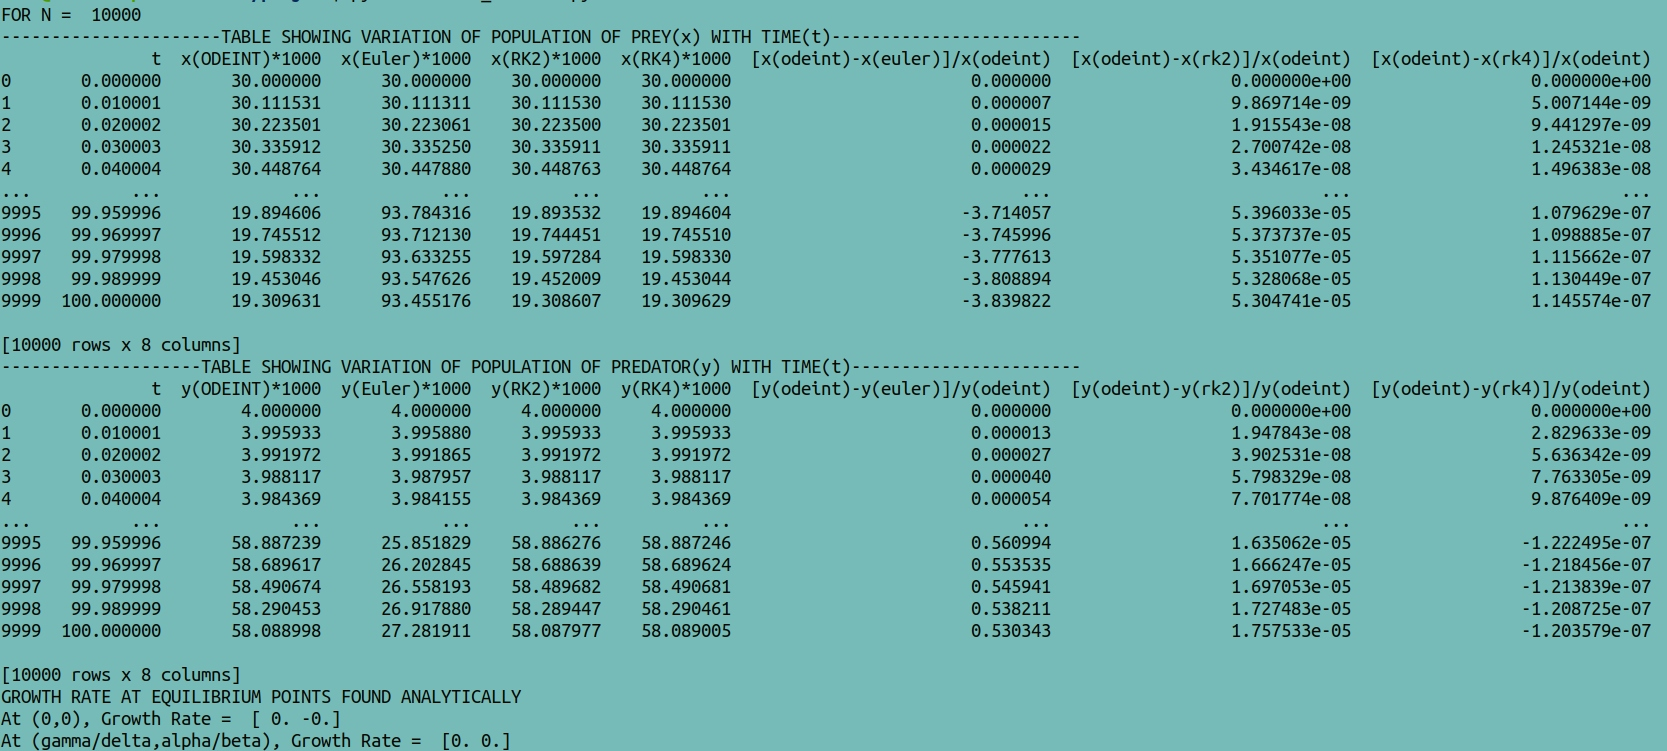
\includegraphics[width=18cm,height=12cm]{table.jpg}
\caption{Table}
\end{figure}






%%%%%%%%%%%%%%%%%%%%%%%%%%%%%%%%%%%%%%
\newpage
\section{Summary}
\label{sec:summary}
\begin{itemize}
    \item This section contains summary of your results or conclusions
    \item It should also include our experience and what you have learnt in this project
    \item Length should be 300- 500 words 
\end{itemize}

\bibliography{ref} % the file ref.bib contains all references in bibtex style
\bibliographystyle{ieeetr}
%%%%%%%%%%%%%%%%%%%%%%%%%%%%%%%
\newpage 
\appendix
\section{Programs}
Python Program including numerical methods impementation and data generation for graph plotting
\begin{lstlisting}[language=Python, caption=Python example]

import numpy as np
import pandas as pd
import matplotlib.pyplot as plt
from scipy import integrate
from matplotlib.animation import FuncAnimation 
import pylab as p

def eqn(t,X, cons):   #Defining Equations 
    x, y = X          #Assigning x,y values 
    alpha,beta,delta,gamma=cons       #Assigning values to parameters 
    dotx = x * (float(alpha) - float(beta) * y)       #dx/dt = alpha*x-beta*x*y
    doty = y * (-float(gamma)+ float(delta) * x)      #dy/dt = delta*x*y-gamma*y
    return np.array([dotx, doty])                     #Returns dx/dt and dy/dt in array 

def eqn1(X, t, alpha, beta, delta, gamma):           #same equations , but taking alpha,beta,delta,gamma parameters as input instead of array
    x, y = X                                         
    dotx = x * (float(alpha) - float(beta) * y)
    doty = y * (-float(gamma)+ float(delta) * x)
    return np.array([dotx, doty])

def Euler(func, X0, tmin,tmax,N, cons):    #Euler Method
    t = np.linspace(tmin,tmax, N)          #Creating array containg N-2 points between tmin and tmax (Basically calculation points)
    dt = t[1] - t[0]                       # calculating step size
    X  = np.zeros([N, len(X0)])            #creating dummy for output array containing x,y values
    X[0] = X0                              #assigning initial values to the output array
    for i in range(N-1):
        X[i+1] = X[i] + func(t[i],X[i],cons) * dt          #Updating values of the dummy array that we created 
    return X,t                                             #returns array of updated values of X and array t

def RK2(func, X0, tmin, tmax,N,cons):         #Runga kutta 2 method
    t = np.linspace(tmin,tmax, N)   #Creating array containg N-2 points between tmin and tmax (Basically calculation points)
    dt = t[1] - t[0]                 # calculating step size
    X  = np.zeros([N, len(X0)])      #creating dummy for output array containing x,y values
    X[0] = X0                        #assigning initial values to the output array
    for i in range(N-1):
        k1 =dt* func(t[i], X[i], cons)
        k2 = dt*func(t[i] + dt,X[i] +  k1 , cons)
        X[i+1] = X[i] + (k1 +  k2 )/2                           #Updating values of the dummy array that we created 
    return X,t                                     #returns array of updated values of X and array t

def RK4(func, X0, tmin, tmax,N,cons):         #Runga kutta 4 method
    t = np.linspace(tmin,tmax, N)   #Creating array containg N-2 points between tmin and tmax (Basically calculation points)
    dt = t[1] - t[0]                 # calculating step size
    X  = np.zeros([N, len(X0)])      #creating dummy for output array containing x,y values
    X[0] = X0                        #assigning initial values to the output array
    for i in range(N-1):
        k1 = func( t[i],X[i], cons)
        k2 = func(t[i] + dt/2.,X[i] + dt/2. * k1, cons)
        k3 = func( t[i] + dt/2., X[i] + dt/2. * k2,cons)
        k4 = func( t[i] + dt, X[i] + dt    * k3,cons)
        X[i+1] = X[i] + dt / 6. * (k1 + 2. * k2 + 2. * k3 + k4)           #Updating values of the dummy array that we created 
    return X,t                                                       #returns array of updated values of X and array t

def V(X,cons):      #Analytic solution of the equation V = delta*x - gamma*ln(x)+beta*y-alpha*ln(y)   
    x,y=X
    alpha,beta,delta,gamma=cons
    return delta*x -gamma*np.log(x)+beta*y-alpha*np.log(y)

def main():
    t = np.linspace(0.,tmax, Nt)      #Creating array containg N-2 points between tmin and tmax (Basically calculation points)
    X0 = [x0, y0]       #Initial conditions
    cons=(alpha,beta,delta,gamma)
    res = integrate.odeint(eqn1, X0, t, args = cons)    #Calling Scipy's odeint function
    x, y = res.T
    Xe = Euler(eqn, X0,0.,tmax,Nt,cons)    #calling Euler
    x1,y1=Xe[0].T
    Xr2 = RK2(eqn, X0,0.,tmax,Nt,cons)      #calling RK2
    x2,y2=Xr2[0].T
    Xr4 = RK4(eqn, X0,0.,tmax,Nt,cons)       #calling RK4
    x3,y3=Xr4[0].T

    xee=[];yee=[];xer2=[];yer2=[];xer4=[];yer4=[]               #Creating empty lists for appending values of abs(odeint-numrical method(euler/rk2/rk4))/odeint
    for i in range(len(x)):                               #comparing our results of Euler,RK2,RK4 with Scipy's ODEint for finding error
        xee.append((x[i]-x1[i])/x[i])
        yee.append((y[i]-y1[i])/y[i])
        xer2.append((x[i]-x2[i])/x[i])
        yer2.append((y[i]-y2[i])/y[i])
        xer4.append((x[i]-x3[i])/x[i])
        yer4.append((y[i]-y3[i])/y[i])              #appending values 
    V_data = V(X=[x3,y3],cons=cons)
    return (t,x,x1,x2,x3,y,y1,y2,y3,xee,yee,xer2,yer2,xer4,yer4,V_data) 

x0 = 30;y0 = 4        # (*1000) INITIAL CONDITIONS     
alpha = 0.453;beta = 0.0205;gamma = 0.790;delta = 0.0229;tmax = 100        #Assigning values of parameters
N_arr=[1000,10000,100000,1000000]                #array for different number of steps

for Nt in N_arr:                                 #calculations for different N and storing values in csv files
    k=main()
    t,x,x1,x2,x3,y,y1,y2,y3,xee,yee,xer2,yer2,xer4,yer4,V_data=k
    DataOut111 = np.column_stack((t,x,x1,x2,x3,y,y1,y2,y3,xee,yee,xer2,yer2,xer4,yer4,V_data))
    if Nt==1000:
        np.savetxt('data_1000.csv', DataOut111,delimiter=',') 
    elif Nt==10000:
        np.savetxt('data_10000.csv', DataOut111,delimiter=',') 
    elif Nt==100000:
        np.savetxt('data_100000.csv', DataOut111,delimiter=',') 
    elif Nt==1000000:
        np.savetxt('data_1000000.csv', DataOut111,delimiter=',') 

Nt=10000
G=main()
t,x,x1,x2,x3,y,y1,y2,y3,xee,yee,xer2,yer2,xer4,yer4,V_data=G
print("FOR N = ",Nt)
print("----------------------TABLE SHOWING VARIATION OF POPULATION OF PREY(x) WITH TIME(t)-------------------------")
data={"t":t,"x(ODEINT)*1000":x ,"x(Euler)*1000":x1,"x(RK2)*1000":x2,"x(RK4)*1000":x3,"[x(odeint)-x(euler)]/x(odeint)":xee,"[x(odeint)-x(rk2)]/x(odeint)":xer2,"[x(odeint)-x(rk4)]/x(odeint)":xer4}
print(pd.DataFrame(data))
print("--------------------TABLE SHOWING VARIATION OF POPULATION OF PREDATOR(y) WITH TIME(t)-----------------------")
data={"t":t,"y(ODEINT)*1000":y ,"y(Euler)*1000":y1,"y(RK2)*1000":y2,"y(RK4)*1000":y3,"[y(odeint)-y(euler)]/y(odeint)":yee,"[y(odeint)-y(rk2)]/y(odeint)":yer2,"[y(odeint)-y(rk4)]/y(odeint)":yer4}
print(pd.DataFrame(data))

X_e1 = np.array([     0 ,  0])                   #Equilibrium condition 1
X_e2 = np.array([ gamma/delta, alpha/beta])      #Equilibrium condition 2                                   
print("GROWTH RATE AT EQUILIBRIUM POINTS FOUND ANALYTICALLY")
print("At (0,0), Growth Rate = ",eqn1(X_e1,t,alpha,beta,delta,gamma))
print("At (gamma/delta,alpha/beta), Growth Rate = ",eqn1(X_e2,t,alpha,beta,delta,gamma))

#Plotting Trajectories and direction fields
values  = np.linspace(1,5, 5)                          
X_f1 = np.array([ int(gamma/delta), int(alpha/beta)])
vcolors = plt.cm.autumn_r(np.linspace(0.1, 0.9, len(values)))  # colors for each trajectory
h1=[];h2=[]
for v, col in zip(values, vcolors):
    X0 = v * X_f1                             # starting point
    X = integrate.odeint(eqn1, X0, t, args = (alpha, beta, delta, gamma))     
    plt.plot( X[:,0], X[:,1], lw=3.5, color=col, label='X0=(%.f, %.f)' % ( X0[0], X0[1]) )
    plt.legend()
    h1.append(X0[0])
    h2.append(X0[1])

ymax = plt.ylim(ymin=0)[1]                    # get axis limits
xmax = plt.xlim(xmin=0)[1]
nb_points   = 30

x = np.linspace(0, xmax, nb_points)
y = np.linspace(0, ymax, nb_points)

X1 , Y1  = p.meshgrid(x, y)    # create a grid     
DX1, DY1 = eqn1([X1,Y1], t, alpha, beta, delta, gamma)               # compute growth rate on the grid
M = (np.hypot(DX1, DY1))                           # Norm of the growth rate 
M[ M == 0] = 1.                              # Avoid zero division errors 
DX1 /= M                                        # Normalize each arrows
DY1 /= M

plt.title('Trajectories and direction fields',fontsize=22,c="r")
plt.scatter(h1,h2,color="black",marker="*",s=300,label="Initial Conditions")
Q = plt.quiver(X1, Y1, DX1, DY1, M, pivot='mid', cmap=p.cm.jet)
plt.xlabel('Number of prey (*1000)',fontsize=19,c="green")
plt.ylabel('Number of predator (*1000)',fontsize=19,c="green")
plt.legend()
plt.grid()
plt.xlim(0, xmax)
plt.ylim(0, ymax)
plt.show()

#ANIMATION
fig = plt.figure()
ax1 = plt.subplot(2, 1, 1)
ax2 = plt.subplot(2, 1, 2)
data_skip = 200

def init_func():
    ax1.clear()
    ax2.clear()
    ax1.set_xlabel('Time ')
    ax1.set_ylabel('[Prey(red) & Predator(green)]*1000')
    ax2.set_xlabel('Prey (*1000)')
    ax2.set_ylabel('Predator (*1000)')
    ax1.set_xlim((t[0], t[-1]))
    ax1.set_ylim((0, 85))
    ax1.grid()
    ax2.set_xlim((5,85))
    ax2.set_ylim((0,70))
    ax2.grid()

def update_plot(i):
    ax1.plot(t[i:i+data_skip], x3[i:i+data_skip], color='k')
    ax1.scatter(t[i], x3[i], marker='o', color='r',label="prey")
    ax1.plot(t[i:i+data_skip], y3[i:i+data_skip], color='k')
    ax1.scatter(t[i], y3[i], marker='o', color='green',label="predator")
    ax2.plot(x3[i:i+data_skip], y3[i:i+data_skip], color='k')
    ax2.scatter(x3[i], y3[i], marker='o', color='magenta')

anim = FuncAnimation(fig,
                     update_plot,
                     frames=np.arange(0, len(t), data_skip),
                     init_func=init_func,
                     interval=1)

anim.save('animation_LotVol.gif', dpi=150, fps=10, writer='ffmpeg')


\end{lstlisting}
\newpage
\section*{Programs for Plotting}
\begin{lstlisting}[language=Gnuplot, caption=Plotting example]
#Euler for diff h
set term pngcairo enhanced size 1280,1024
set datafile separator ","
set output 'euler_diff_h.png'
set border linewidth 2

set multiplot layout 2,1 
set key top left Left box title 
set xlabel 'Time(Years)' 
set ylabel 'Population'
set title "Euler Method(Predator) for different step sizes"  font "enhanced [,20]"
plot "Euler_data.csv" u 1:2 title "n = 1000" , "Euler_data.csv" u 4:5 title "n=10000" , "Euler_data.csv" u 7:8 title "n = 100000", "Euler_data.csv" u 10:11 title "n = 1000000"
set title "Euler Method(Prey) for different step sizes"  font "enhanced [,20]"
plot "Euler_data.csv" u 1:3 title "n = 1000" , "Euler_data.csv" u 4:6 title "n=10000" , "Euler_data.csv" u 7:9 title "n = 100000", "Euler_data.csv" u 10:12 title "n = 1000000"
unset multiplot

#Plotting time v/s population
set term pngcairo enhanced size 1280,1024


set datafile separator ","
set output 'time_vs_population.png'
set border linewidth 2

set style line 1 linecolor rgb 'blue' linetype 1 linewidth 8
set style line 1 linecolor rgb 'green' linetype 1 linewidth 8
set multiplot layout 2,2 #title "Time v/s Population" font "enhanced [,30]"
set key top left Left box title 
set xlabel 'Time(Years)' 
set ylabel 'Population'
set title "OdeInt"  font "enhanced [,20]"
plot "test.csv" u 1:2 title "Predator" w l , "test.csv" u 1:6 title "Prey"  w l
set title "Euler Method"  font "enhanced [,20]"
plot "test.csv" u 1:3 title "Predator"  w l, "test.csv" u 1:7  title "Prey" w l
set title "Rk2 Method"  font "enhanced [,20]"
plot "test.csv" u 1:4  title "Predator" w l, "test.csv" u 1:8  title "Prey" w l
set title "Rk4 Method"  font "enhanced [,20]"
plot "test.csv" u 1:5  title "Predator" w l, "test.csv" u 1:9  title "Prey" w l
set title "rk4"

unset multiplot



#Error Plot for predator and prey
set term pngcairo enhanced size 1280,1024
set datafile separator ","
set output 'error_plot.png'
set border linewidth 2

set multiplot layout 2,1 #title "Time v/s Population" font "enhanced [,30]"
set key bottom left Left box title 
set xlabel 'Time(Years)' 
set ylabel 'Absolute Error'
set title "Error Plot(Predator)"  font "enhanced [,20]"
plot "test.csv" u 1:10 pt 4 title "Euler Method" , "test.csv" u 1:13 pt 4 ps 3 title "Rk2 Method" , "test.csv" u 1:15 pt 4 title "Rk4 Method"
set title "Error Plot(Prey)"  font "enhanced [,20]"
plot "test.csv" u 1:11 pt 4 title "Euler Method"  , "test.csv" u 1:13 pt 4 ps 3 title "Rk2 Method" , "test.csv" u 1:15 pt 4 title "Rk4 Method"
unset multiplot
\end{lstlisting}
\newpage 
\section{Contribution of team mates}
\large{\bf {Contribution of "{\it name of partner A}"}}
\begin{itemize}
   \item In Formulation of the problem:  
   \item  In Programming: 
   \item  In Plotting Graphs:
   \item  In Report Writing: 
\end{itemize}
\large{\bf {Contribution of "{\it name of partner B}"}}
\begin{itemize}
   \item In Formulation of the problem:  
   \item  In Programming: 
   \item  In Plotting Graphs:
   \item  In Report Writing:
\end{itemize}
\large{\bf {Contribution of "{\it name of partner C}"}}
\begin{itemize}
   \item In Formulation of the problem:  
   \item  In Programming: 
   \item  In Plotting Graphs:
   \item  In Report Writing: 
\end{itemize}

%%%
\end{document}
